\chapter{Visualisation et alertes}
\label{chap:chap_4}

\section{Collecte et gestion des logs prioritaires en sécurité}

Comme détaillé dans le chapitre précédent, le système de détection d’intrusion (Suricata) génère en continu des journaux relatifs aux activités réseau.  
Ces logs sont collectés et centralisés via syslog-ng, puis transmis à Elasticsearch pour être analysés et visualisés dans Kibana.  
Cette chaîne (Suricata → syslog-ng → Elasticsearch → Kibana) assure la traçabilité complète des événements de sécurité observés lors des cinq scénarios d’intrusion précédemment simulés.

\subsection{Collecte et transfert des journaux}

Les journaux produits par Suricata sont stockés dans le répertoire \path{/var/log/suricata/}.  
On distingue principalement deux fichiers :
\begin{itemize}
  \item \texttt{fast.log} : enregistre les alertes textuelles (lisibles directement dans le terminal) ;
  \item \texttt{eve.json} : contient l’ensemble des événements au format JSON, destiné à être lu par \texttt{syslog-ng} pour transfert vers la base \texttt{Elasticsearch}.
\end{itemize}

Afin de vérifier que le processus de collecte est bien actif, la commande suivante permet d’observer que \texttt{syslog-ng} lit en continu le fichier \texttt{eve.json} :
\begin{verbatim}
sudo lsof /var/log/suricata/eve.json
\end{verbatim}

\begin{figure}[H]
    \centering
    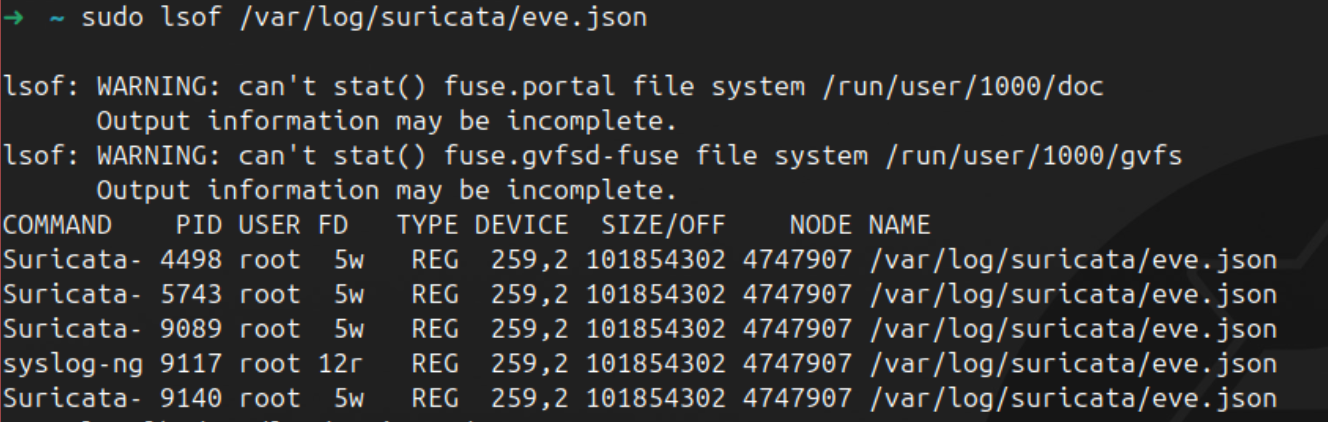
\includegraphics[width=0.9\linewidth]{assets/figures/syslog_ng_evejson.png}
    \caption{Vérification du flux de collecte : \texttt{syslog-ng} lit en continu \texttt{eve.json}.}
    \label{fig:syslog_ng_evejson}
\end{figure}

\subsection{Structure et rotation automatique des logs}

Les fichiers de journaux sont automatiquement gérés par le service logrotate, qui effectue périodiquement une rotation et une compression des anciens fichiers.  
Cela garantit une conservation historique tout en évitant la saturation du disque.

La commande suivante permet de visualiser cette rotation automatique :
\begin{verbatim}
ls -lh /var/log/suricata/
\end{verbatim}

\begin{figure}[H]
    \centering
    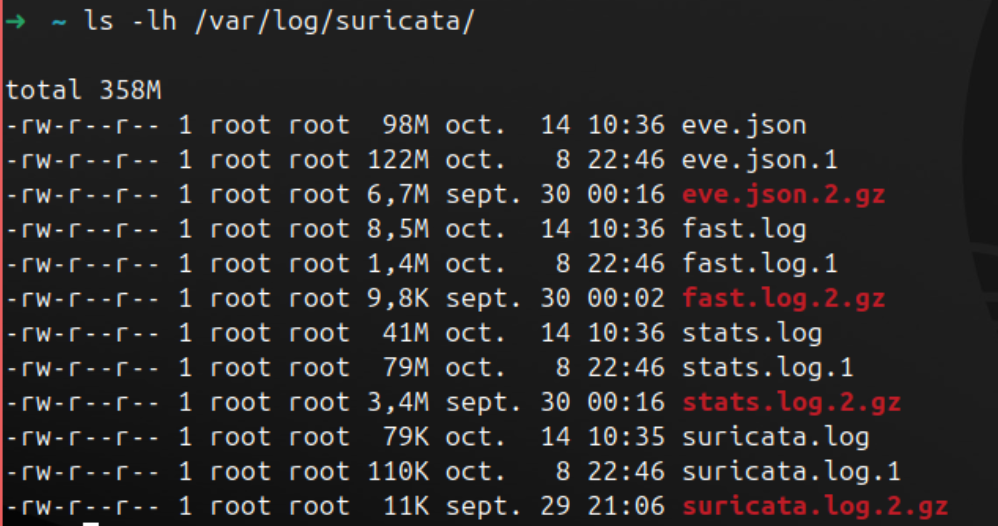
\includegraphics[width=0.75\linewidth]{assets/figures/suricata_logs_rotation.png}
    \caption{Rotation automatique et compression des journaux dans \texttt{/var/log/suricata/}.}
    \label{fig:suricata_logs_rotation}
\end{figure}

Les fichiers actifs portent l’extension \texttt{.log}, tandis que les précédents sont numérotés (\texttt{.log.1}) et les plus anciens compressés (\texttt{.log.2.gz}).  
Cette rotation automatique est essentielle pour maintenir la disponibilité et la fiabilité des logs dans le temps.

\subsection{Corrélation et visualisation dans Kibana}

Les événements issus de Suricata sont ensuite indexés dans Elasticsearch et visualisés dans Kibana Discover.  
Chaque alerte correspond à une signature spécifique (champ \texttt{alert.signature}) générée par l’une des règles locales définies pour les scénarios ICMP, Nmap, SSH, Web Fuzzing et FTP comme on l'a vu dans les chapitres précédents du rapport.

\subsection{Synthèse de la collecte par scénario}

\begin{table}[H]
\centering
\begin{tabular}{|l|l|l|}
\hline
\textbf{Scénario d’intrusion} & \textbf{Type d’événement détecté} & \textbf{Fichiers de logs concernés} \\ \hline
1 — ICMP (Ping) & Trafic ICMP (echo request/reply) & fast.log / eve.json \\ \hline
2 — Scan Nmap & Connexions TCP multiples & fast.log / eve.json \\ \hline
3 — SSH & Connexions répétées sur le port 22 & fast.log / eve.json \\ \hline
4 — Web Fuzzing & Volume élevé de requêtes HTTP & fast.log / eve.json \\ \hline
5 — FTP Anonyme & Connexion au port 21 (anonymous login) & fast.log / eve.json \\ \hline
\end{tabular}
\caption{Correspondance entre les scénarios d’intrusion et les types de logs collectés.}
\label{tab:scen_logs}
\end{table}

\subsection{Justification et intérêt sécurité}

Ce mécanisme de collecte et de gestion centralisée offre plusieurs avantages essentiels :
\begin{itemize}
    \item \textbf{Détection précoce des comportements anormaux}, grâce à la corrélation des alertes entre différents protocoles ;
    \item \textbf{Préservation des preuves techniques} (traçabilité et audit post-incident) ;
    \item \textbf{Hiérarchisation des menaces} via la priorité et le niveau de sévérité des logs ;
    \item \textbf{Surveillance continue et automatique}, assurée par la rotation et la centralisation.
\end{itemize}

\clearpage
\section{Point bonus — Tableau de bord Kibana personnalisé}

\textbf{Objectif :} Créer un tableau de bord Kibana personnalisé afin de visualiser en temps réel les alertes issues de Suricata et de synthétiser les cinq scénarios d'intrusion précédemment mis en œuvre.

\textbf{Procédure de création :}
\begin{enumerate}
    \item Dans Kibana, accéder à \textbf{Analytics → Dashboard → Create new dashboard}.
    \item Ajouter les visualisations sauvegardées depuis la bibliothèque (\texttt{Add from library}), notamment :
    \begin{itemize}
        \item \textbf{KPI – Total alerts} : affiche le nombre total d’alertes détectées ;
        \item \textbf{Alerts over time} : courbe temporelle représentant l’évolution des alertes ;
        \item \textbf{Top alert signatures} : histogramme horizontal illustrant les signatures d’alerte les plus fréquentes ;
    \end{itemize}
\end{enumerate}

\textbf{Résultat :}  
La figure \ref{fig:kibana_dashboard_final} illustre le tableau de bord final.  
Celui-ci offre une vue d’ensemble en temps réel sur l’activité réseau détectée par l’IDS, tout en permettant à l’administrateur de filtrer dynamiquement par signature, adresse IP ou période temporelle.

\begin{figure}[H]
    \centering
    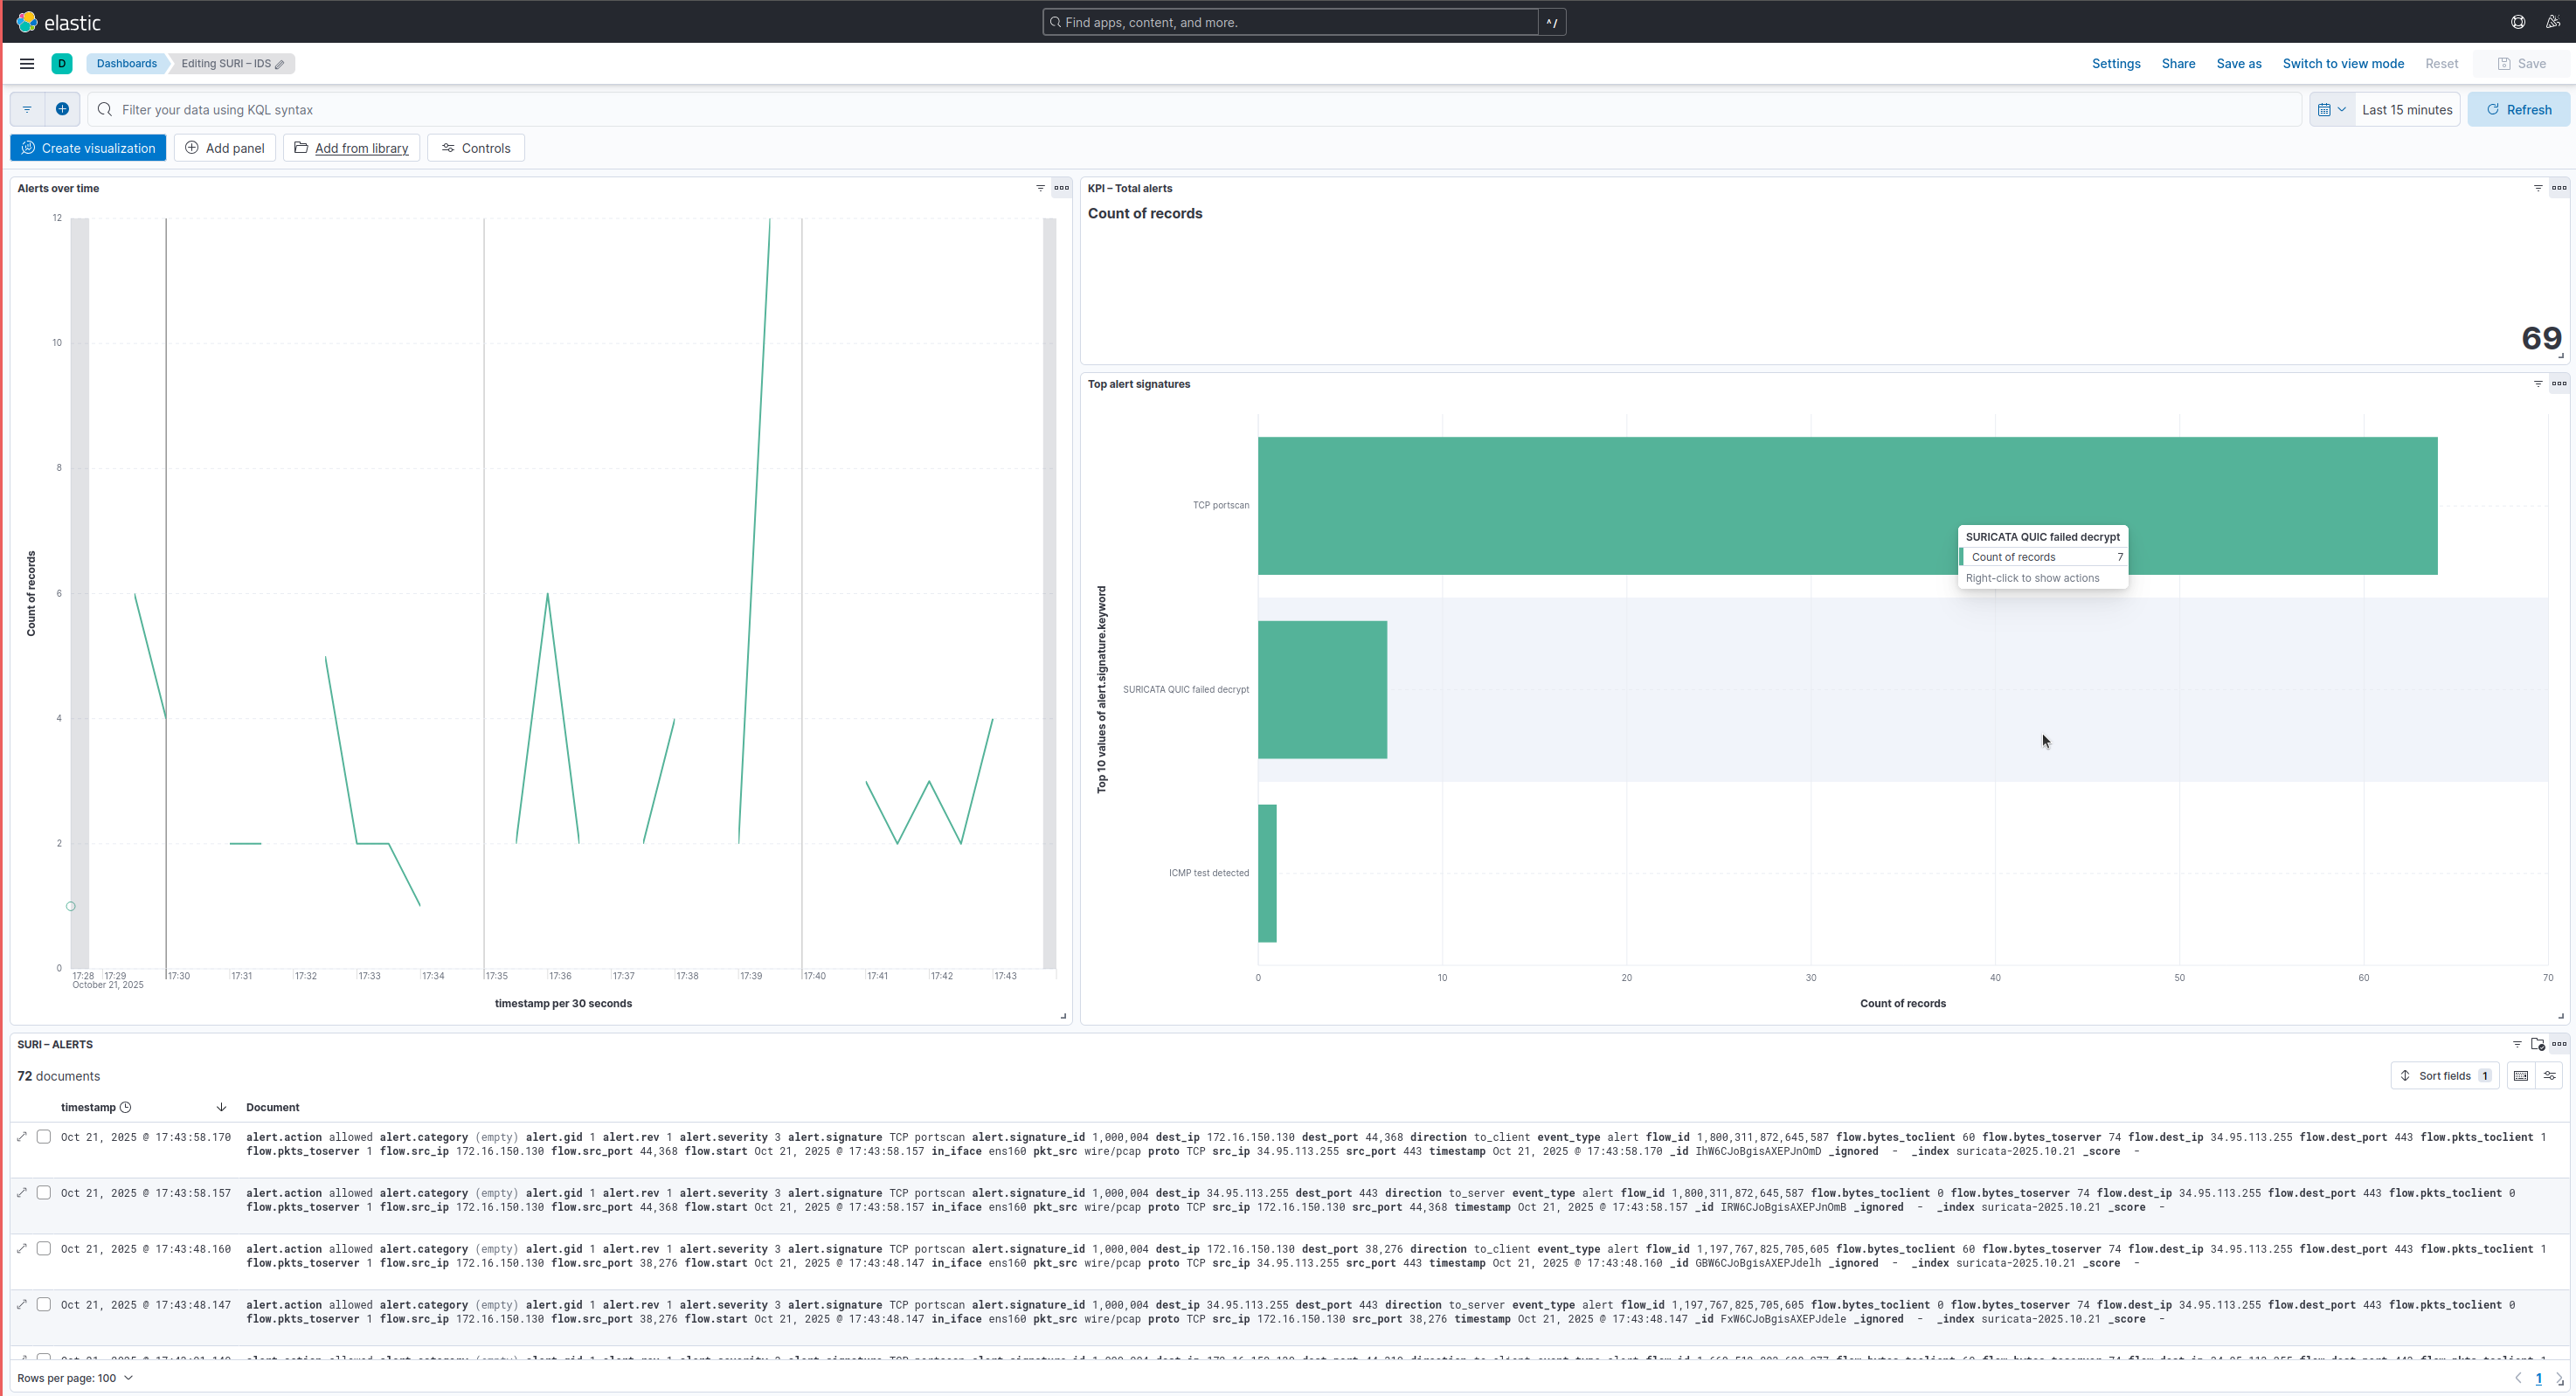
\includegraphics[width=0.6\linewidth]{assets/figures/kibana_dashboard_final.png}
    \caption{Tableau de bord Kibana personnalisé regroupant les visualisations issues des cinq scénarios de détection Suricata.}
    \label{fig:kibana_dashboard_final}
\end{figure}

\clearpage
\section{Point bonus — Automatisation des alertes Slack}

Afin d'améliorer la réactivité du système de détection, un script Python a été mis en place pour envoyer automatiquement les alertes Suricata vers un canal Slack dédié.

Chaque nouvelle alerte écrite dans le fichier \texttt{/var/log/suricata/eve.json} est analysée en temps réel.  
Les informations principales (signature, IP source et destination, niveau de sévérité) sont ensuite transmises via un \textit{webhook} Slack, permettant à l’administrateur d’être notifié instantanément sur mobile ou desktop.

\begin{figure}[H]
    \centering
    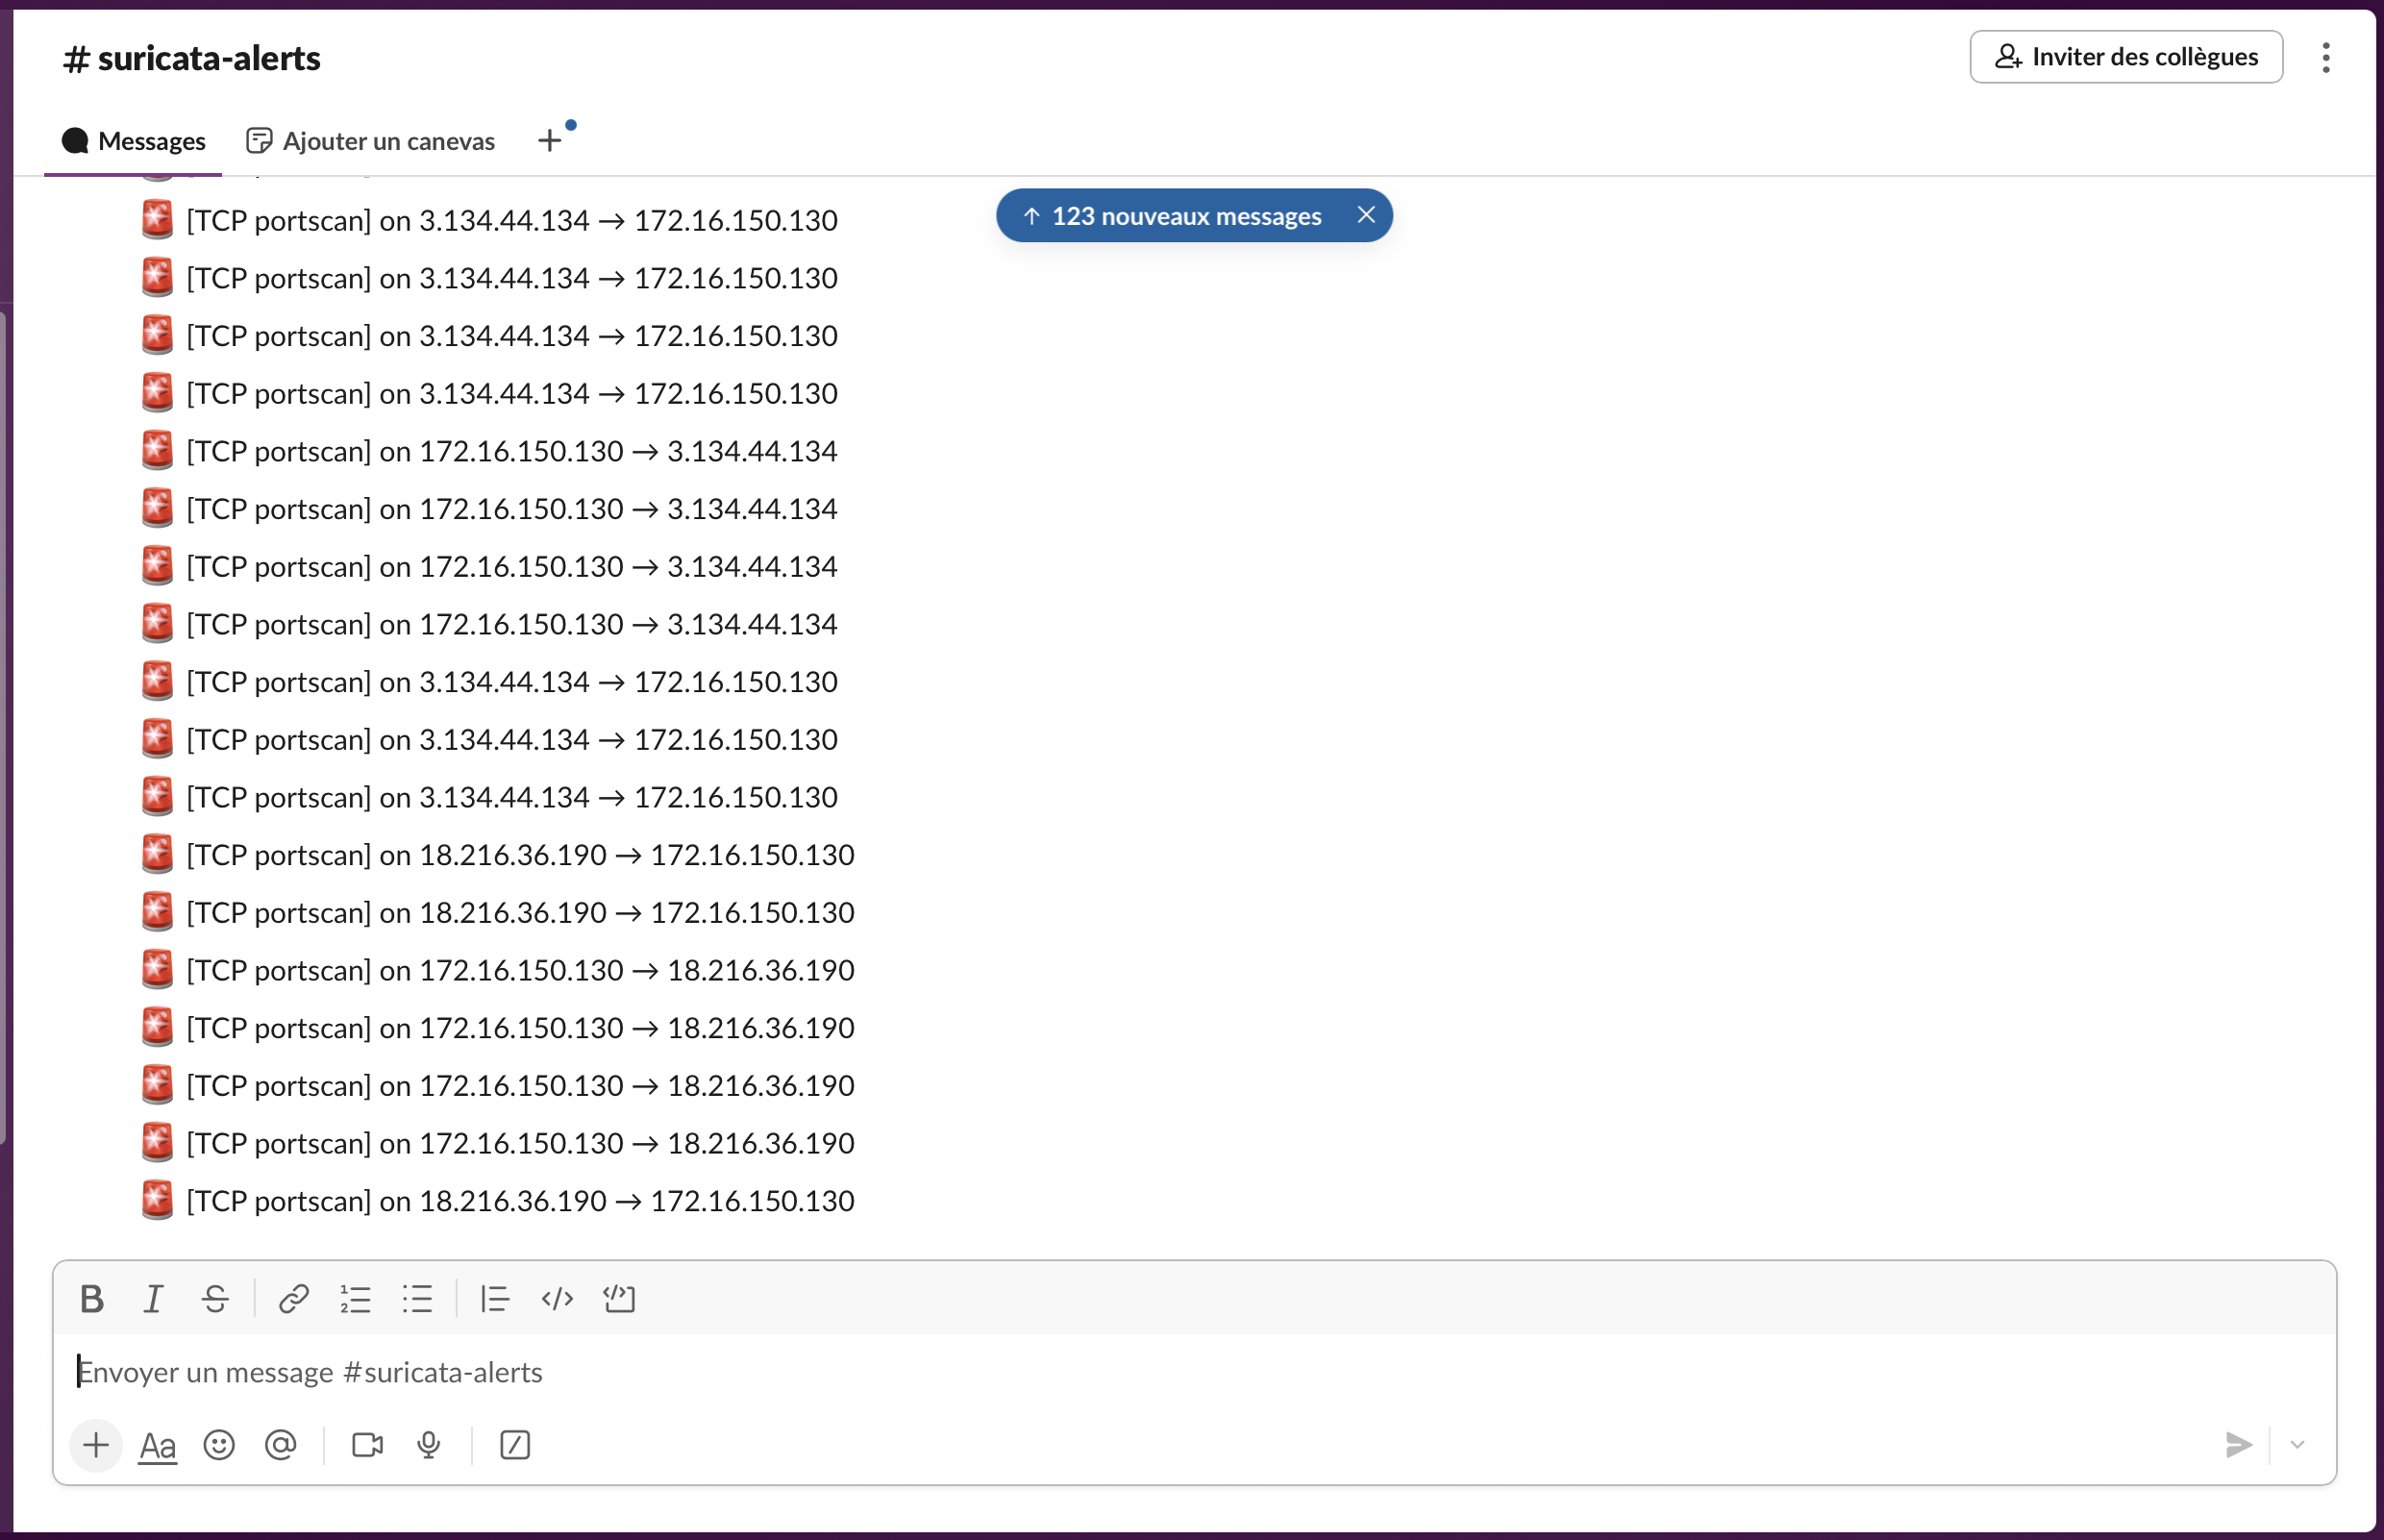
\includegraphics[width=0.9\linewidth]{assets/figures/slack_alert_example.png}
    \caption{Notification automatique d'une alerte Suricata envoyée sur Slack.}
    \label{fig:slack_alert_example}
\end{figure}

Cette automatisation transforme la solution IDS en un véritable outil de supervision active, 
capable de prévenir immédiatement l’administrateur en cas d’incident de sécurité.

\clearpage
\section{Point bonus — Schéma d'architecture (Mermaid)}

La figure~\ref{fig:arch_suricata} présente l’architecture de la solution :
Suricata écoute simultanément sur \texttt{ens160} et \texttt{lo} ; les événements sont écrits dans \texttt{/var/log/suricata/eve.json}, collectés par \texttt{syslog-ng} puis indexés dans \texttt{Elasticsearch}. Les tableaux de bord Kibana exploitent ces données pour l’investigation. Les alertes critiques sont parallèlement envoyées vers Slack via un \textit{webhook}. La rotation des journaux (\texttt{logrotate}) garantit la maîtrise du stockage.

\begin{figure}[H]
  \centering
  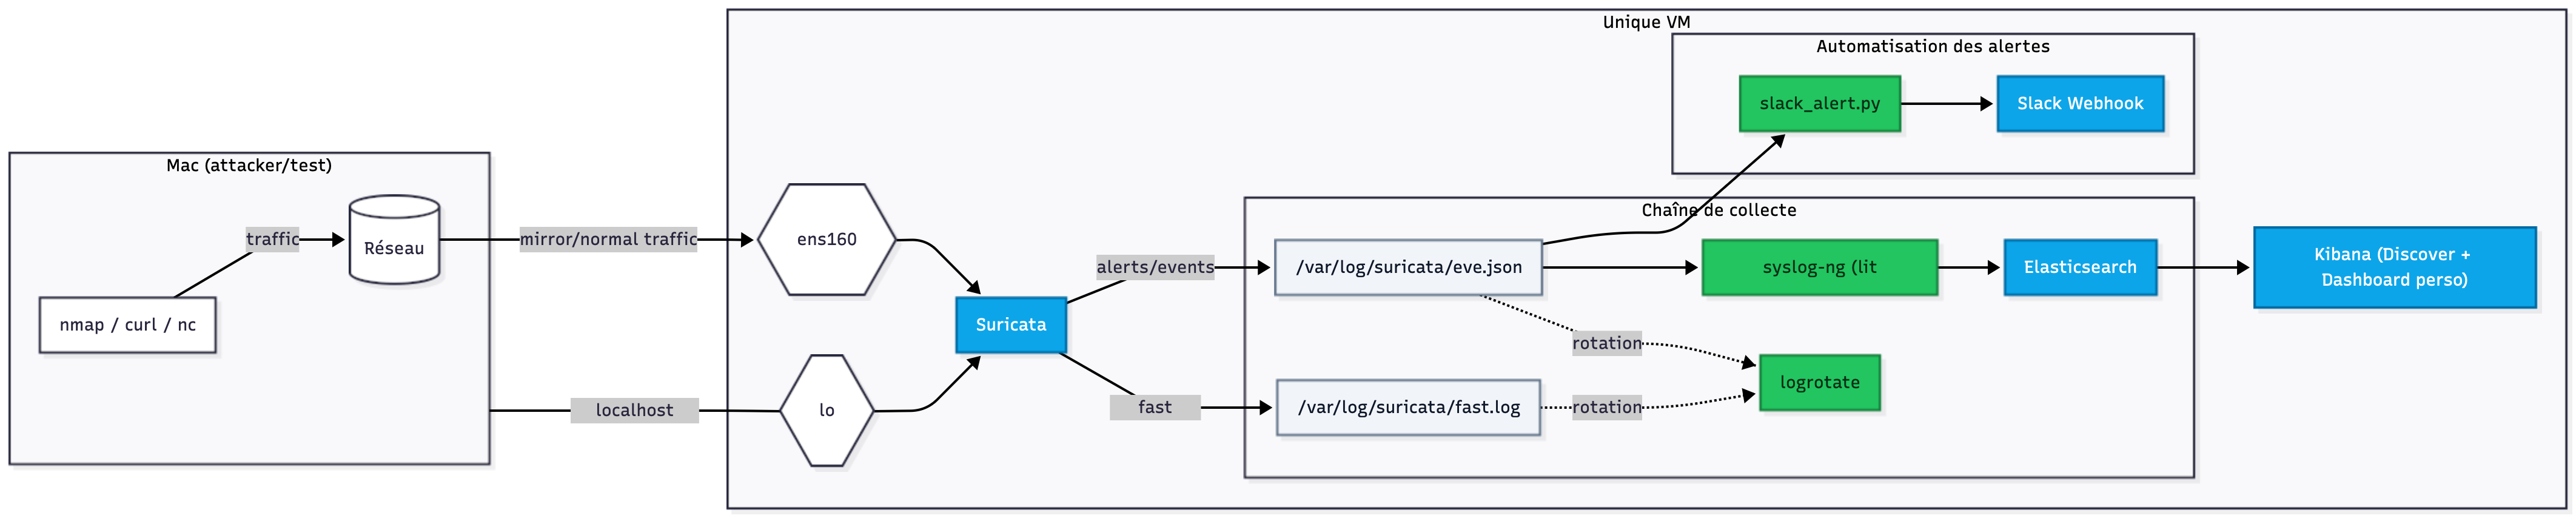
\includegraphics[width=\linewidth]{assets/figures/arch_suricata_stack.png}
  \caption{Chaîne de collecte et supervision : Suricata $\rightarrow$ syslog-ng $\rightarrow$ Elasticsearch $\rightarrow$ Kibana, avec envoi d'alertes Slack et rotation des logs.}
  \label{fig:arch_suricata}
\end{figure}